%%%%%%%%%%%%%%%%%%%%%%%%%%%%%%%%%%%%%%%%%%  不使用 authblk 包制作标题  %%%%%%%%%%%%%%%%%%%%%%%%%%%%%%%%%%%%%%%%%%%%%%
%-------------------------------PPT Title-------------------------------------
\title{\rm{VASP}的主体流程}
%-----------------------------------------------------------------------------

%----------------------------Author & Date------------------------------------
%\author[\textrm{Jun\_Jiang}]{姜\;\;骏\inst{}} %[]{} (optional, use only with lots of authors)
%% - Give the names in the same order as the appear in the paper.
%% - Use the \inst{?} command only if the authors have different
%%   affiliation.
\institute[BCC]{\inst{}%
%\institute[Gain~Strong]{\inst{}%
\vskip -20pt 北京市计算中心}
%\vskip -20pt {\large 格致斯创~科技}}
\date[\today] % (optional, should be abbreviation of conference name)
{%	{\fontsize{6.2pt}{4.2pt}\selectfont{\textcolor{blue}{E-mail:~}\url{jiangjun@bcc.ac.cn}}}
\vskip 45 pt {\fontsize{8.2pt}{6.2pt}\selectfont{%清华大学\;\;物理系% 报告地点
	\vskip 5 pt \textrm{2022.07.01}}}
}

%% - Either use conference name or its abbreviation
%% - Not really information to the audience, more for people (including
%%   yourself) who are reading the slides onlin%%   yourself) who are reading the slides onlin%%   yourself) who are reading the slides onlineee
%%%%%%%%%%%%%%%%%%%%%%%%%%%%%%%%%%%%%%%%%%%%%%%%%%%%%%%%%%%%%%%%%%%%%%%%%%%%%%%%%%%%%%%%%%%%%%%%%%%%%%%%%%%%%%%%%%%%%

\subject{}
% This is only inserted into the PDF information catalog. Can be left
% out.
%\maketitle
\frame
{
%	\frametitle{\fontsize{9.5pt}{5.2pt}\selectfont{\textcolor{orange}{“高通量并发式材料计算算法与软件”年度检查}}}
\titlepage
}
%-----------------------------------------------------------------------------

%------------------------------------------------------------------------------列出全文 outline ---------------------------------------------------------------------------------
%\section*{}
%\frame[allowframebreaks]
%{
%  \frametitle{Outline}
%%  \frametitle{\textcolor{mycolor}{\secname}}
%  \tableofcontents%[current,currentsection,currentsubsection]
%}
%%在每个section之前列出全部Outline
%%类似的在每个subsection之前列出全部Outline是\AtBeginSubsection[]
%\AtBeginSection[]
%{
%  \frame<handout:0>%[allowframebreaks]
%  {
%    \frametitle{Outline}
%%全部Outline中,本部分加亮
%    \tableofcontents[current,currentsection]
%  }
%}

%-----------------------------------------------PPT main Body------------------------------------------------------------------------------------
\small
%\frame[allowframebreaks]
\begin{frame}[allowframebreaks]{\textrm{VASP}的主程序结构}
\begin{figure}[h!]
\vskip 10pt
\centering
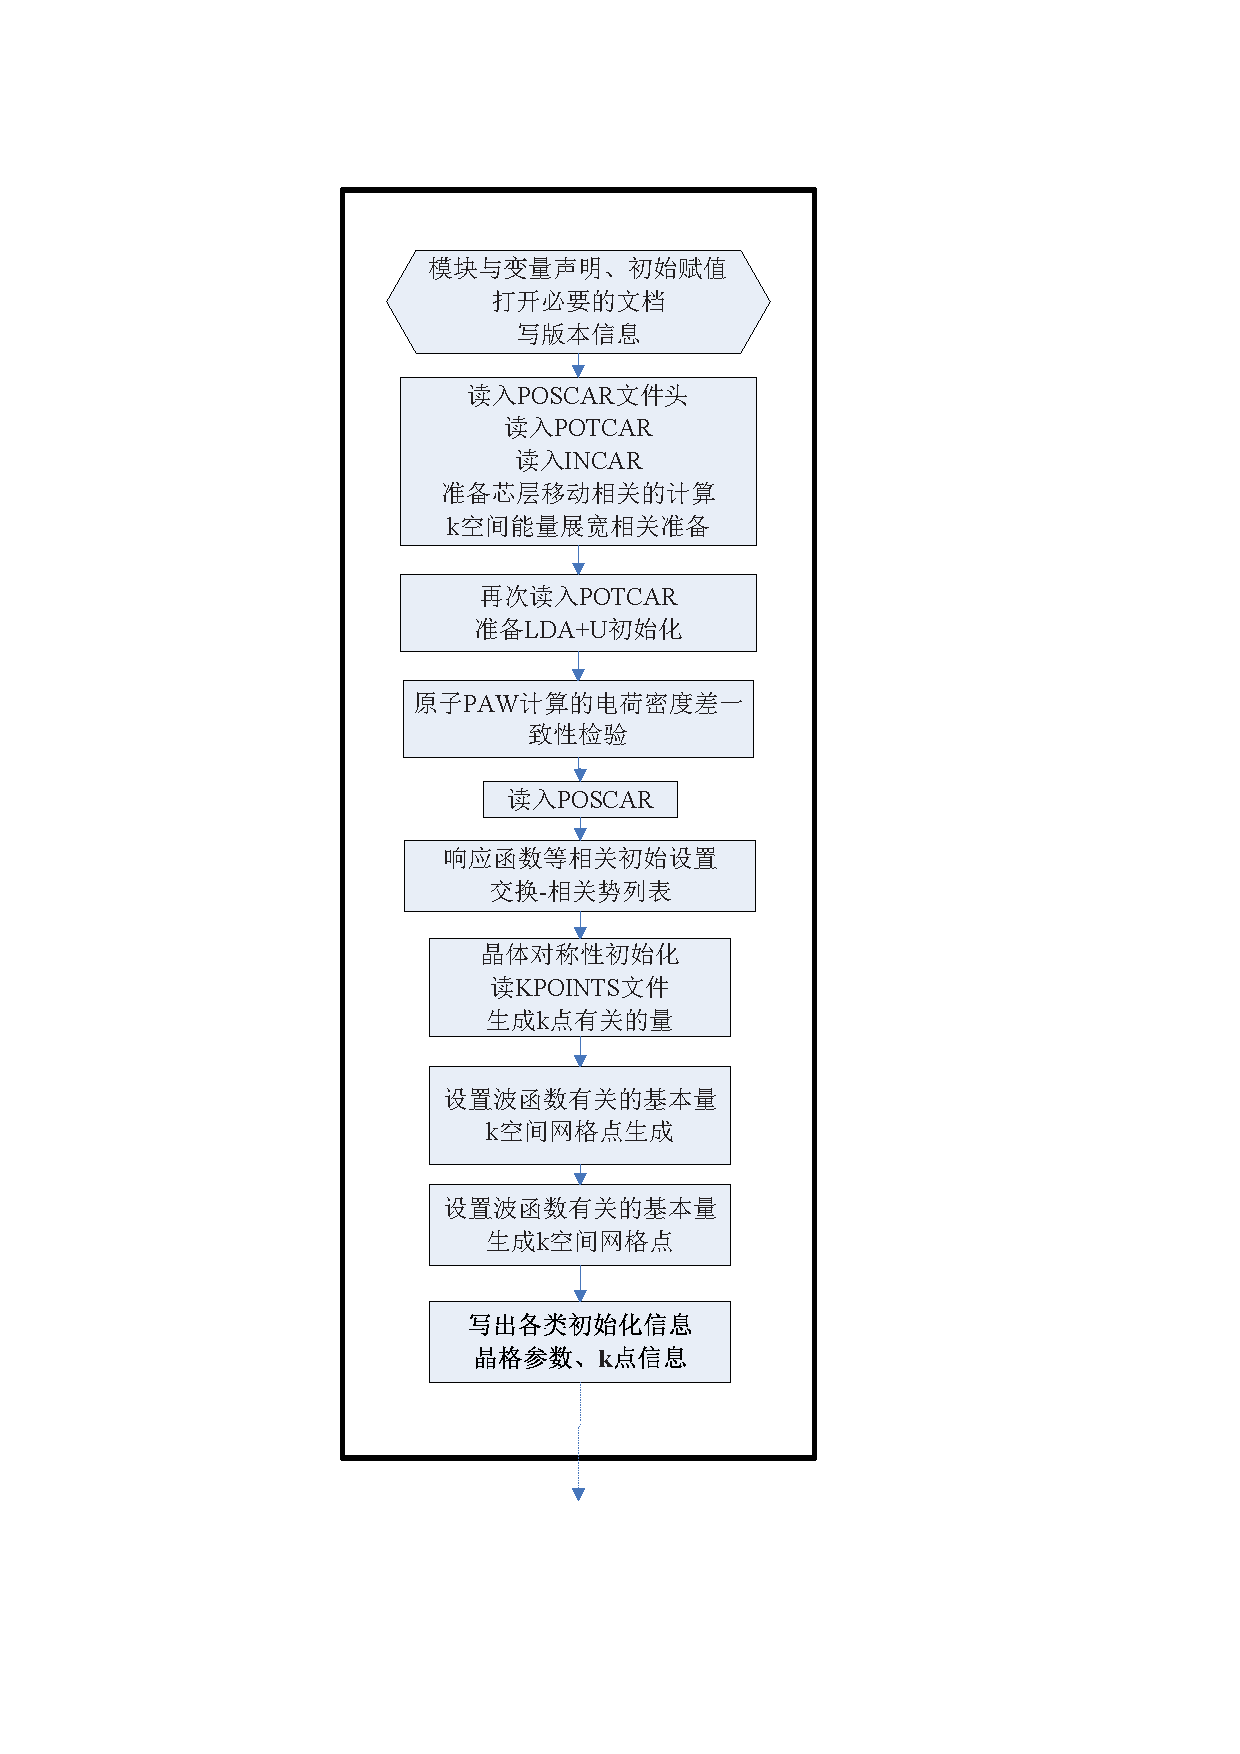
\includegraphics[height=2.35in,width=4.0in,viewport=0 360 562 720,clip]{Figures/VASP_main_Flow-1.png}
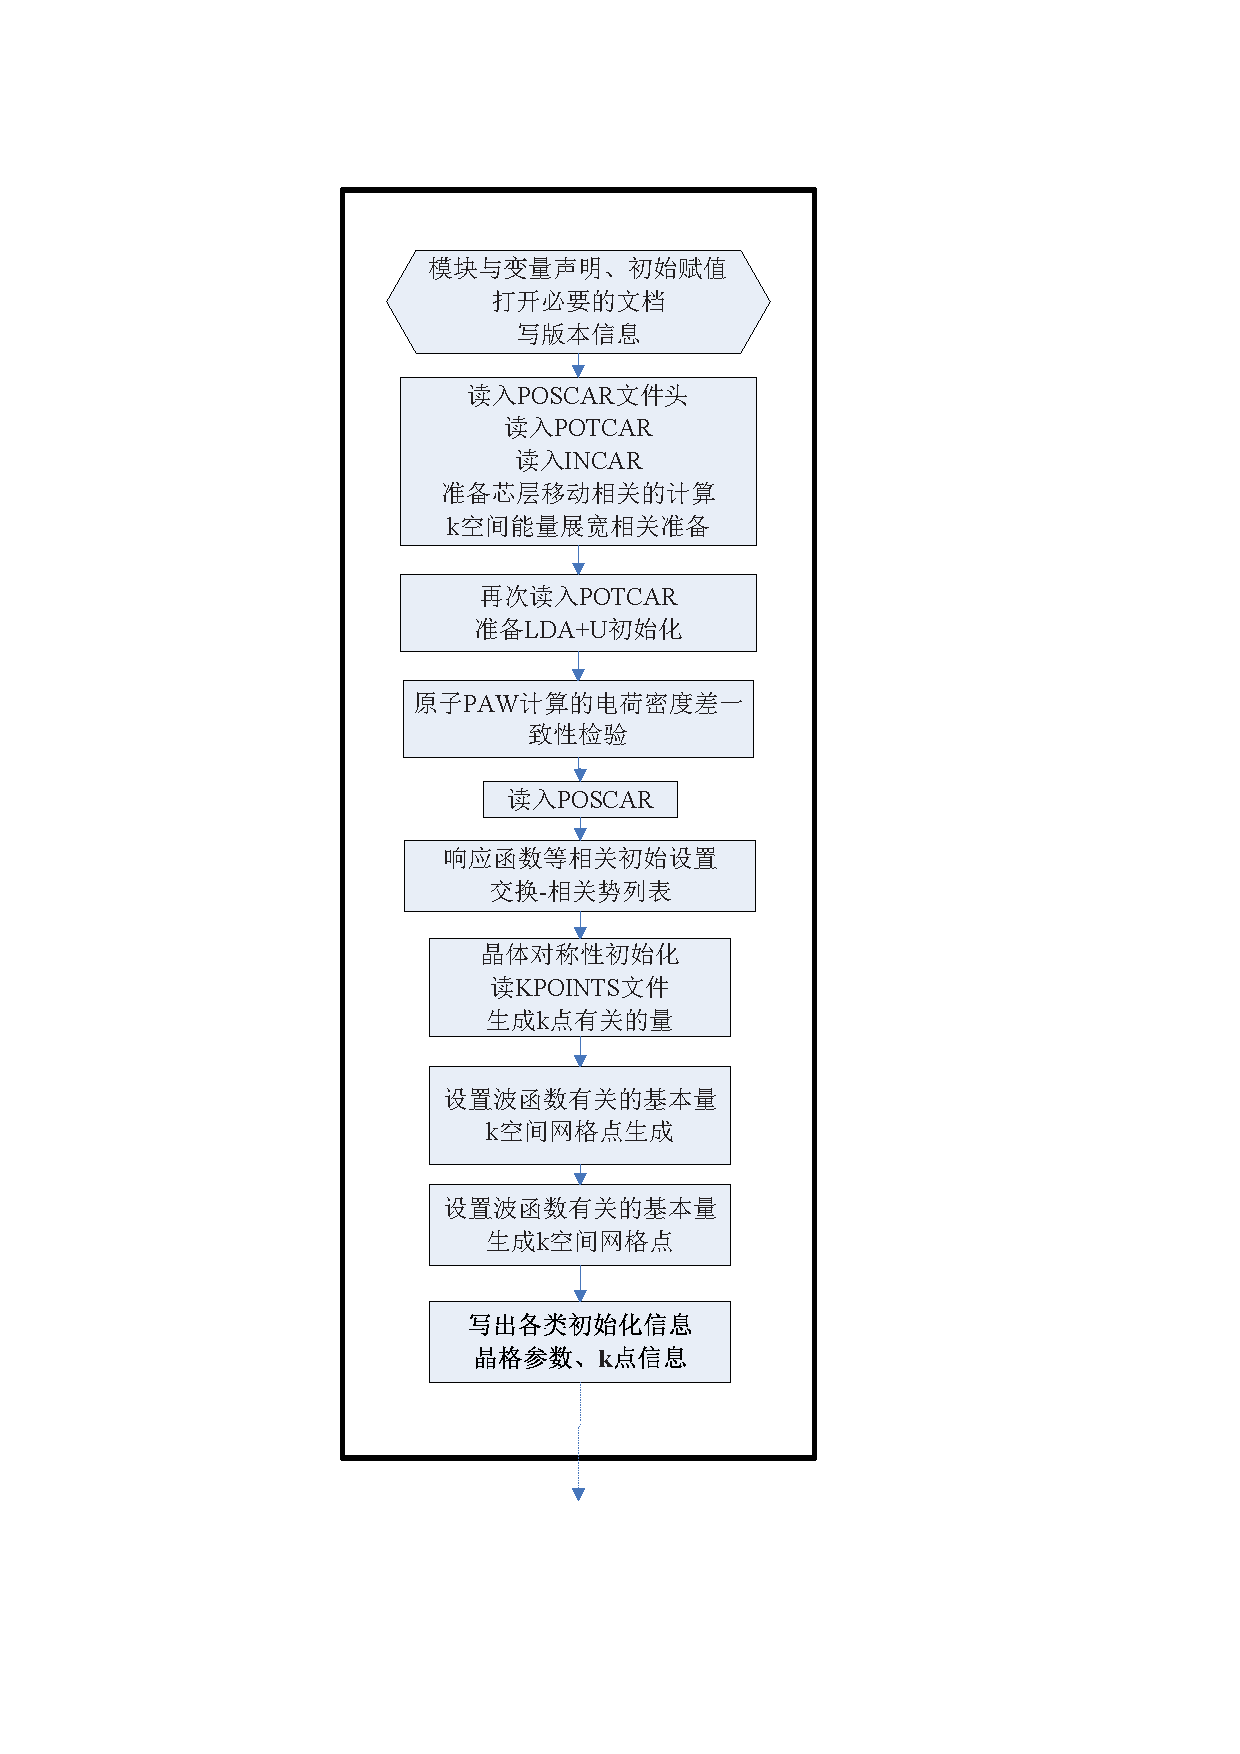
\includegraphics[height=2.35in,width=4.0in,viewport=0 0 562 360,clip]{Figures/VASP_main_Flow-1.png}
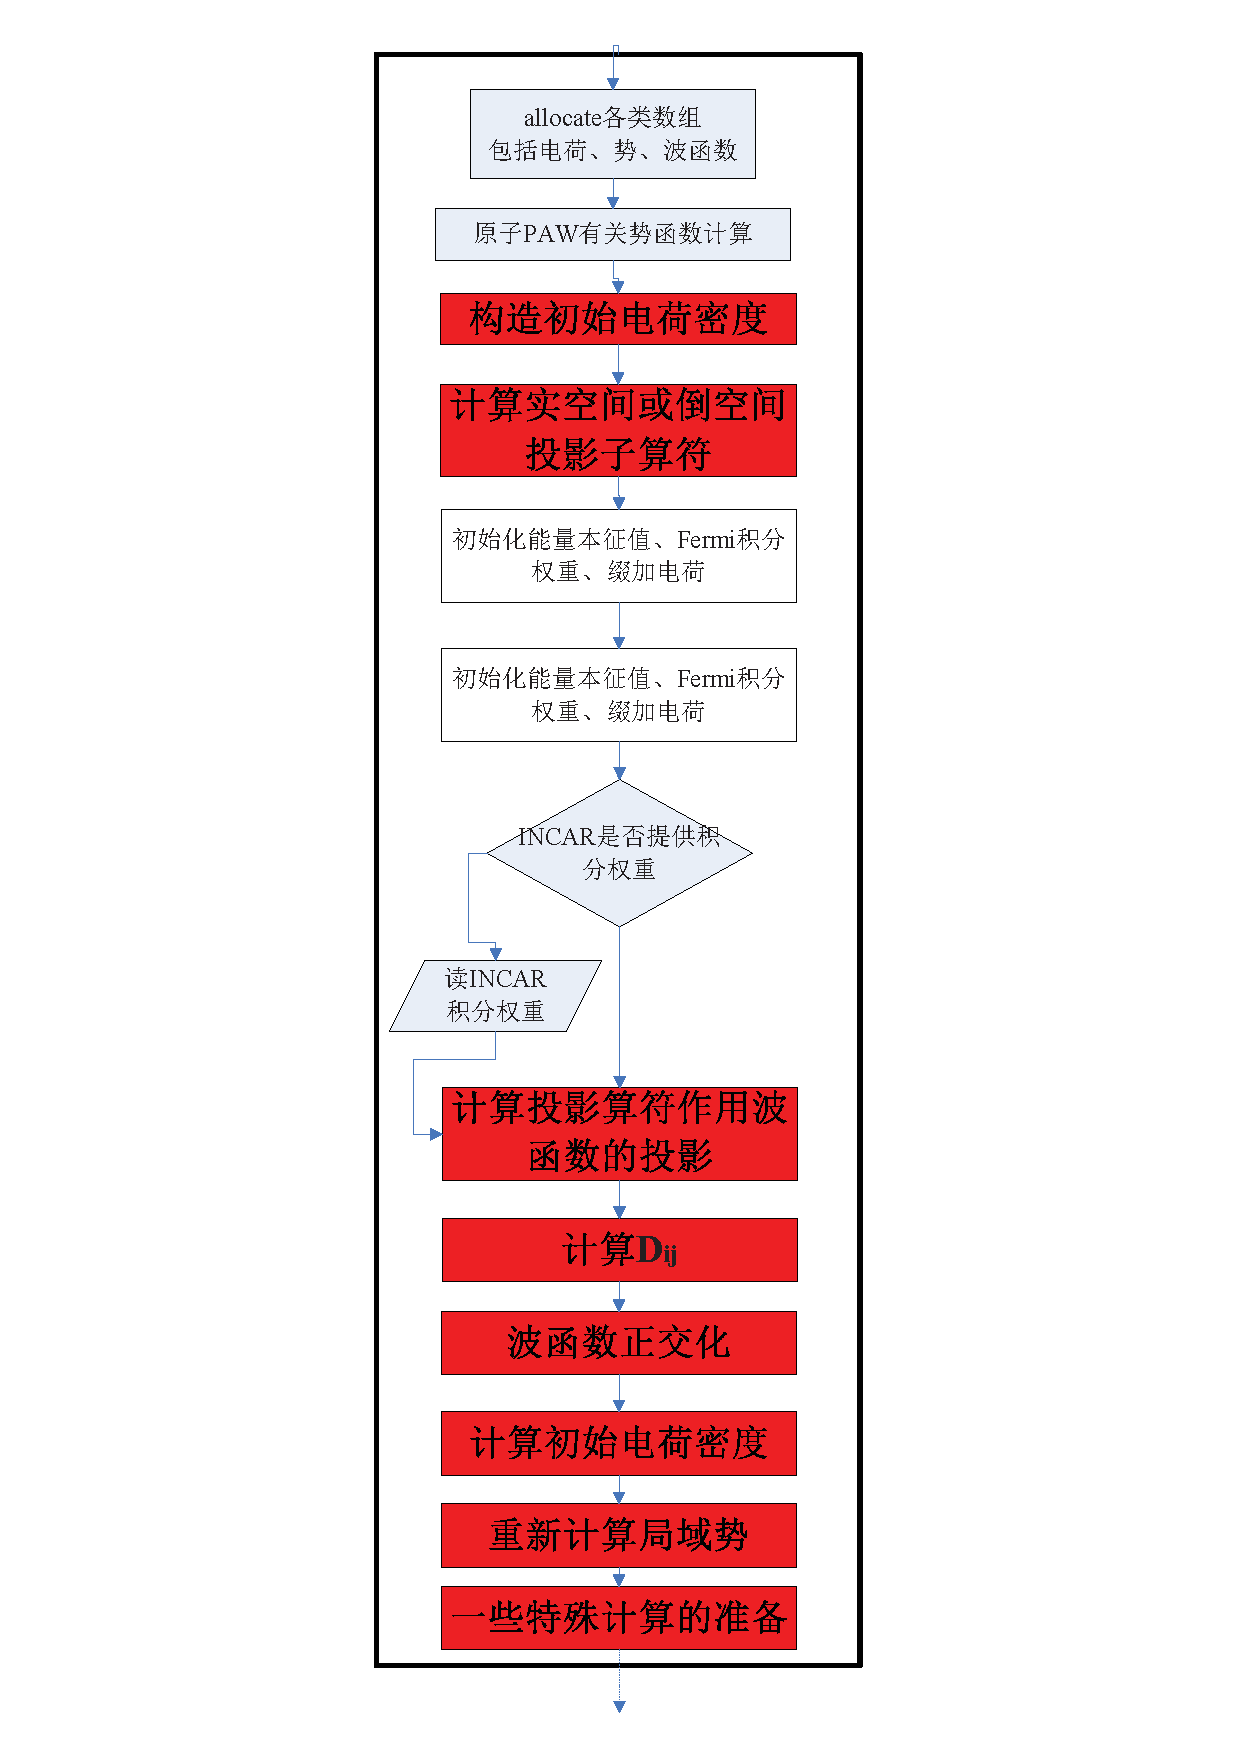
\includegraphics[height=2.35in,width=4.0in,viewport=0 370 562 720,clip]{Figures/VASP_main_Flow-2.png}
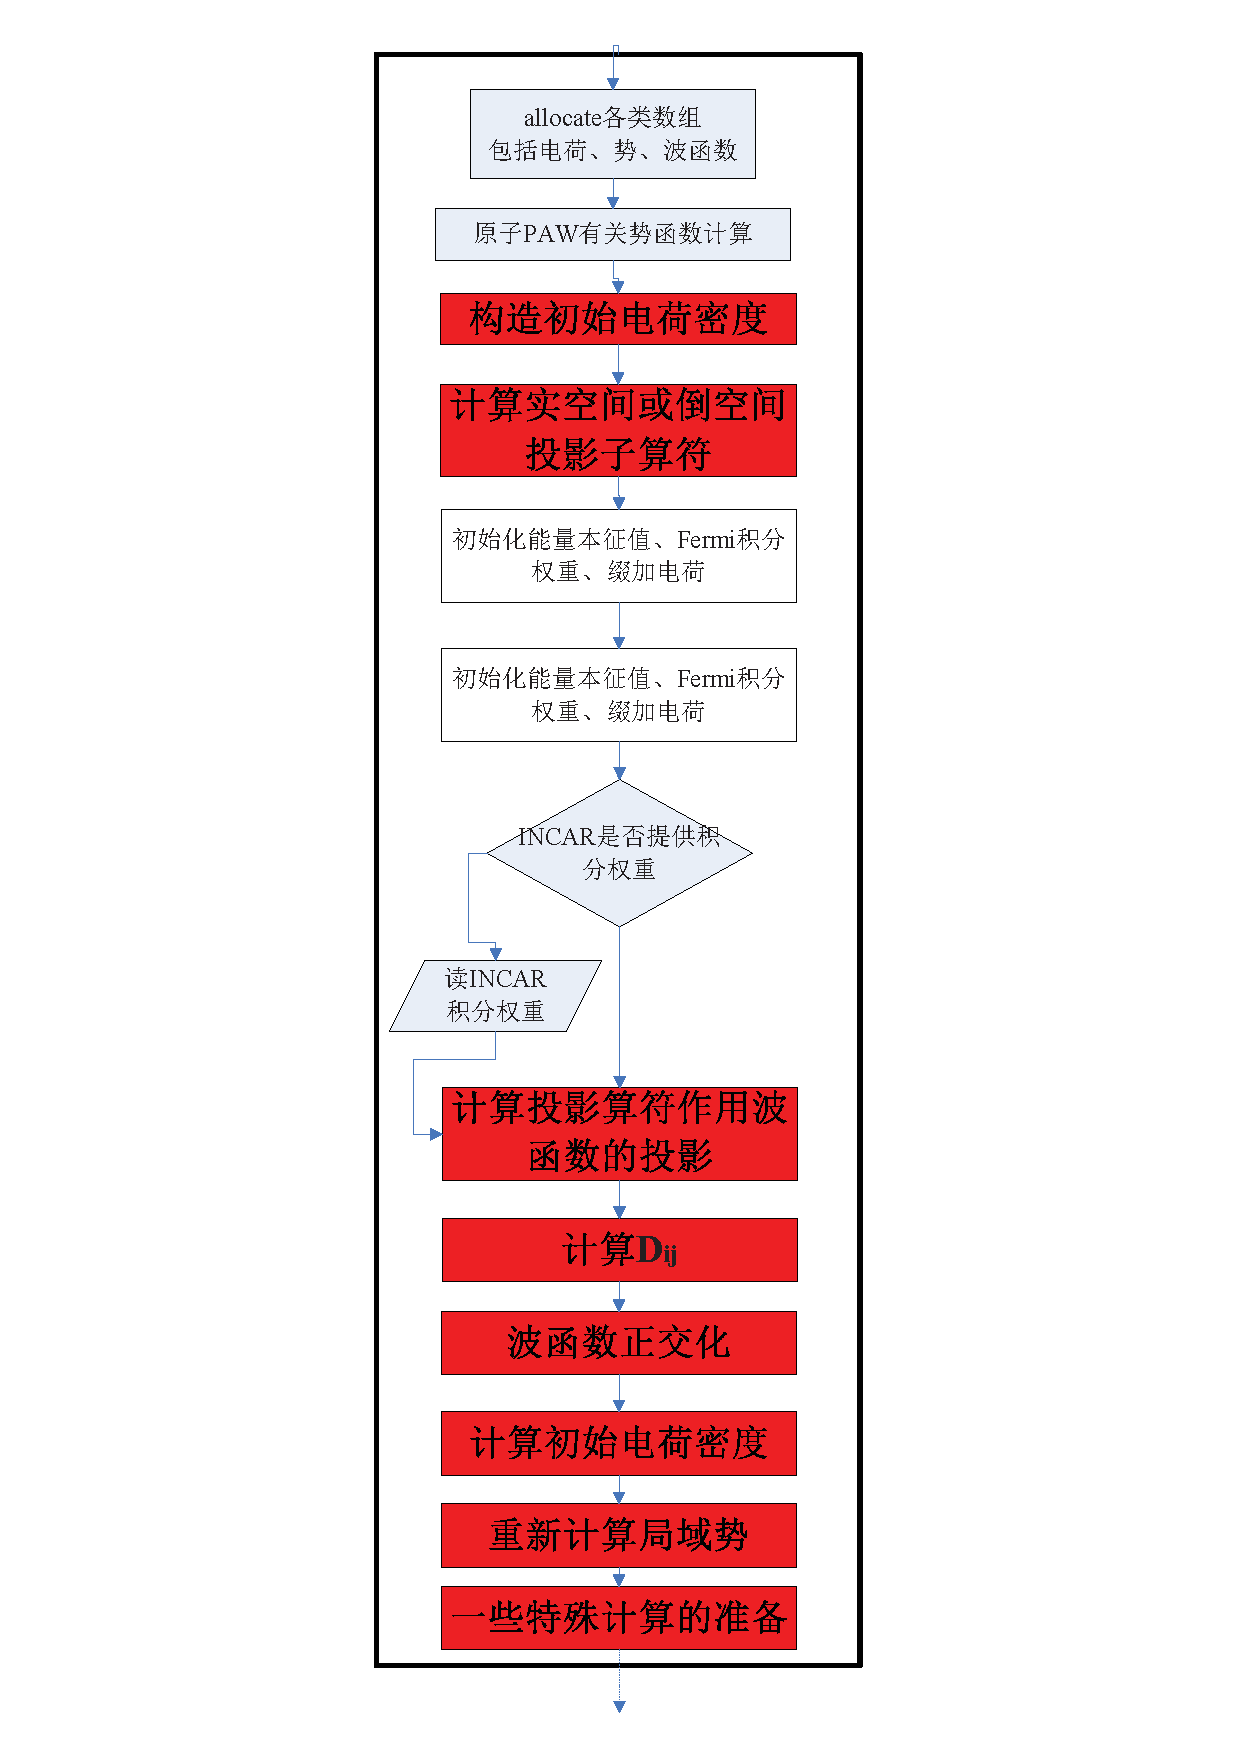
\includegraphics[height=2.30in,width=4.0in,viewport=0 0 562 370,clip]{Figures/VASP_main_Flow-2.png}
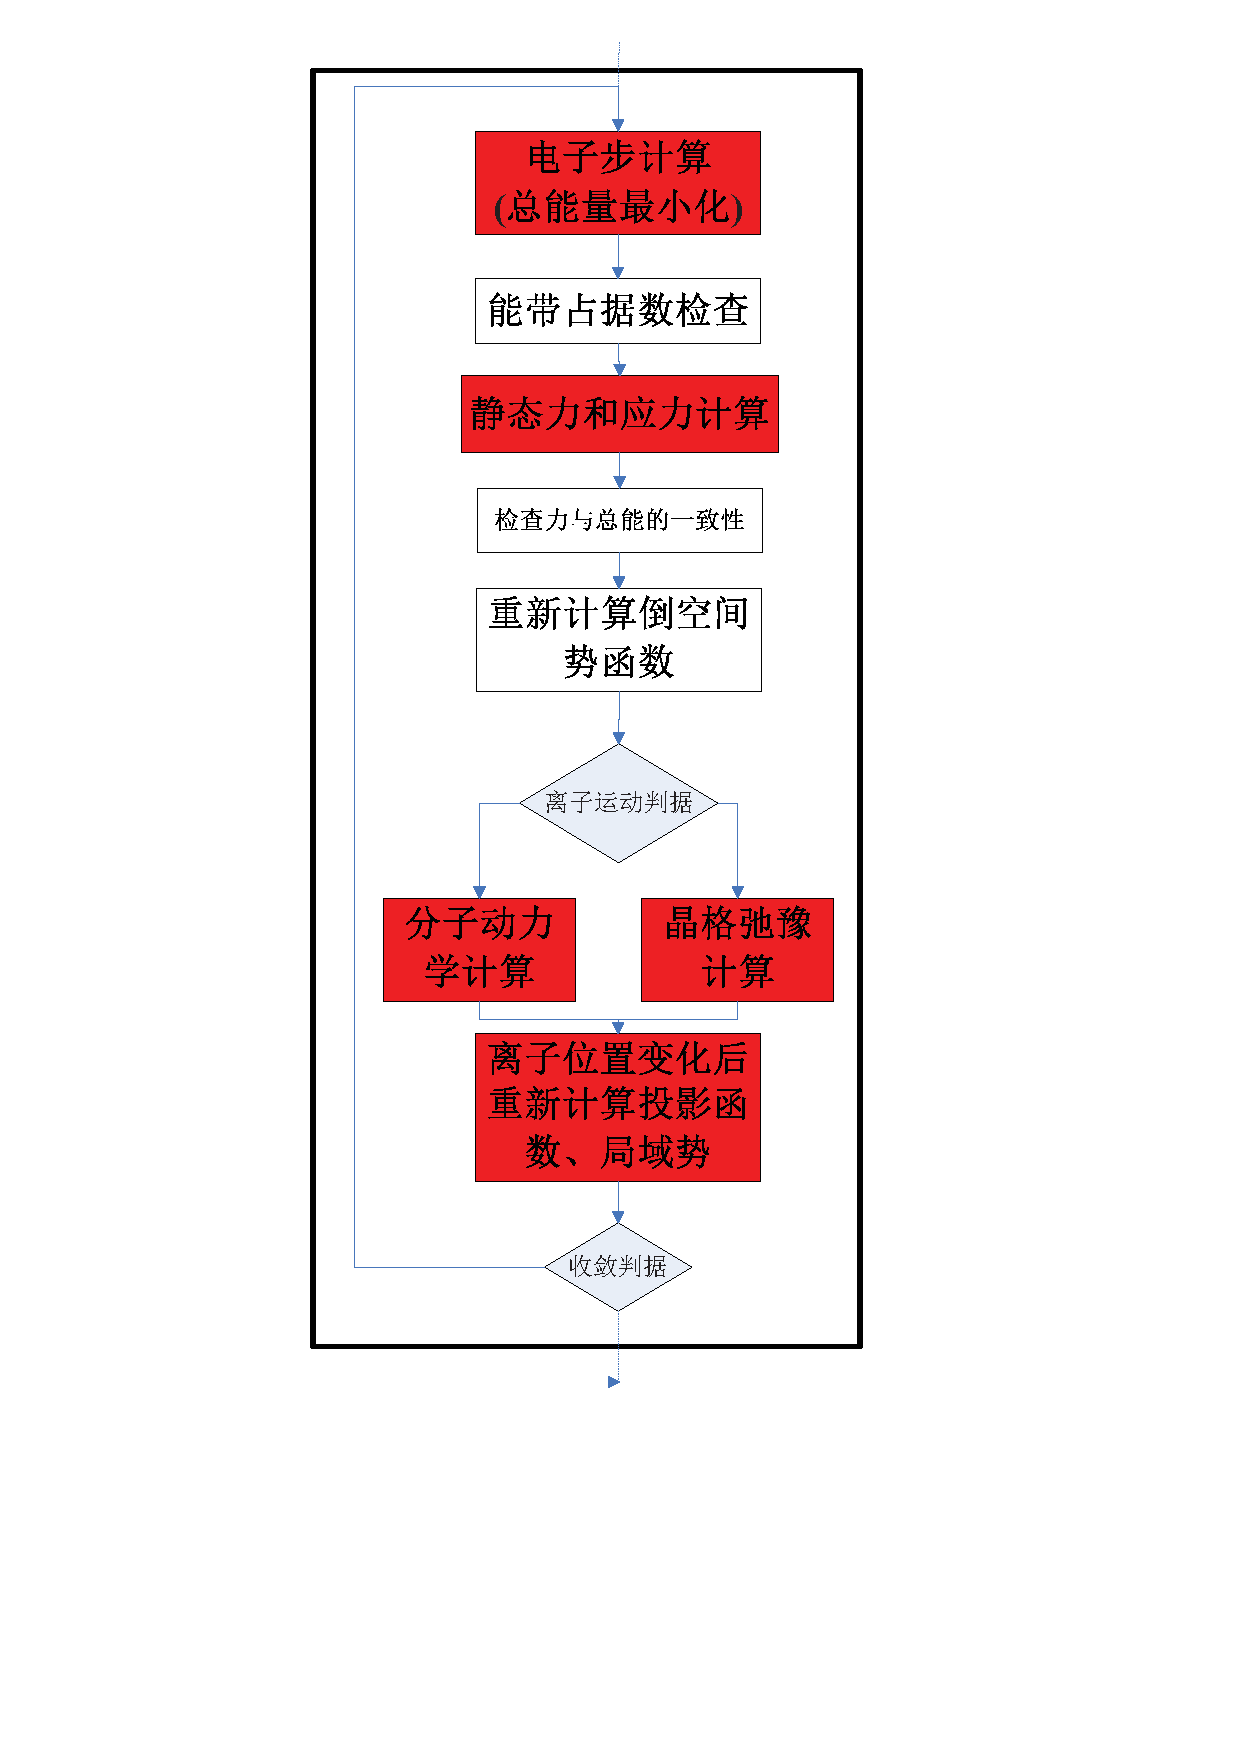
\includegraphics[height=2.35in,width=4.0in,viewport=0 350 562 680,clip]{Figures/VASP_main_Flow-3.png}
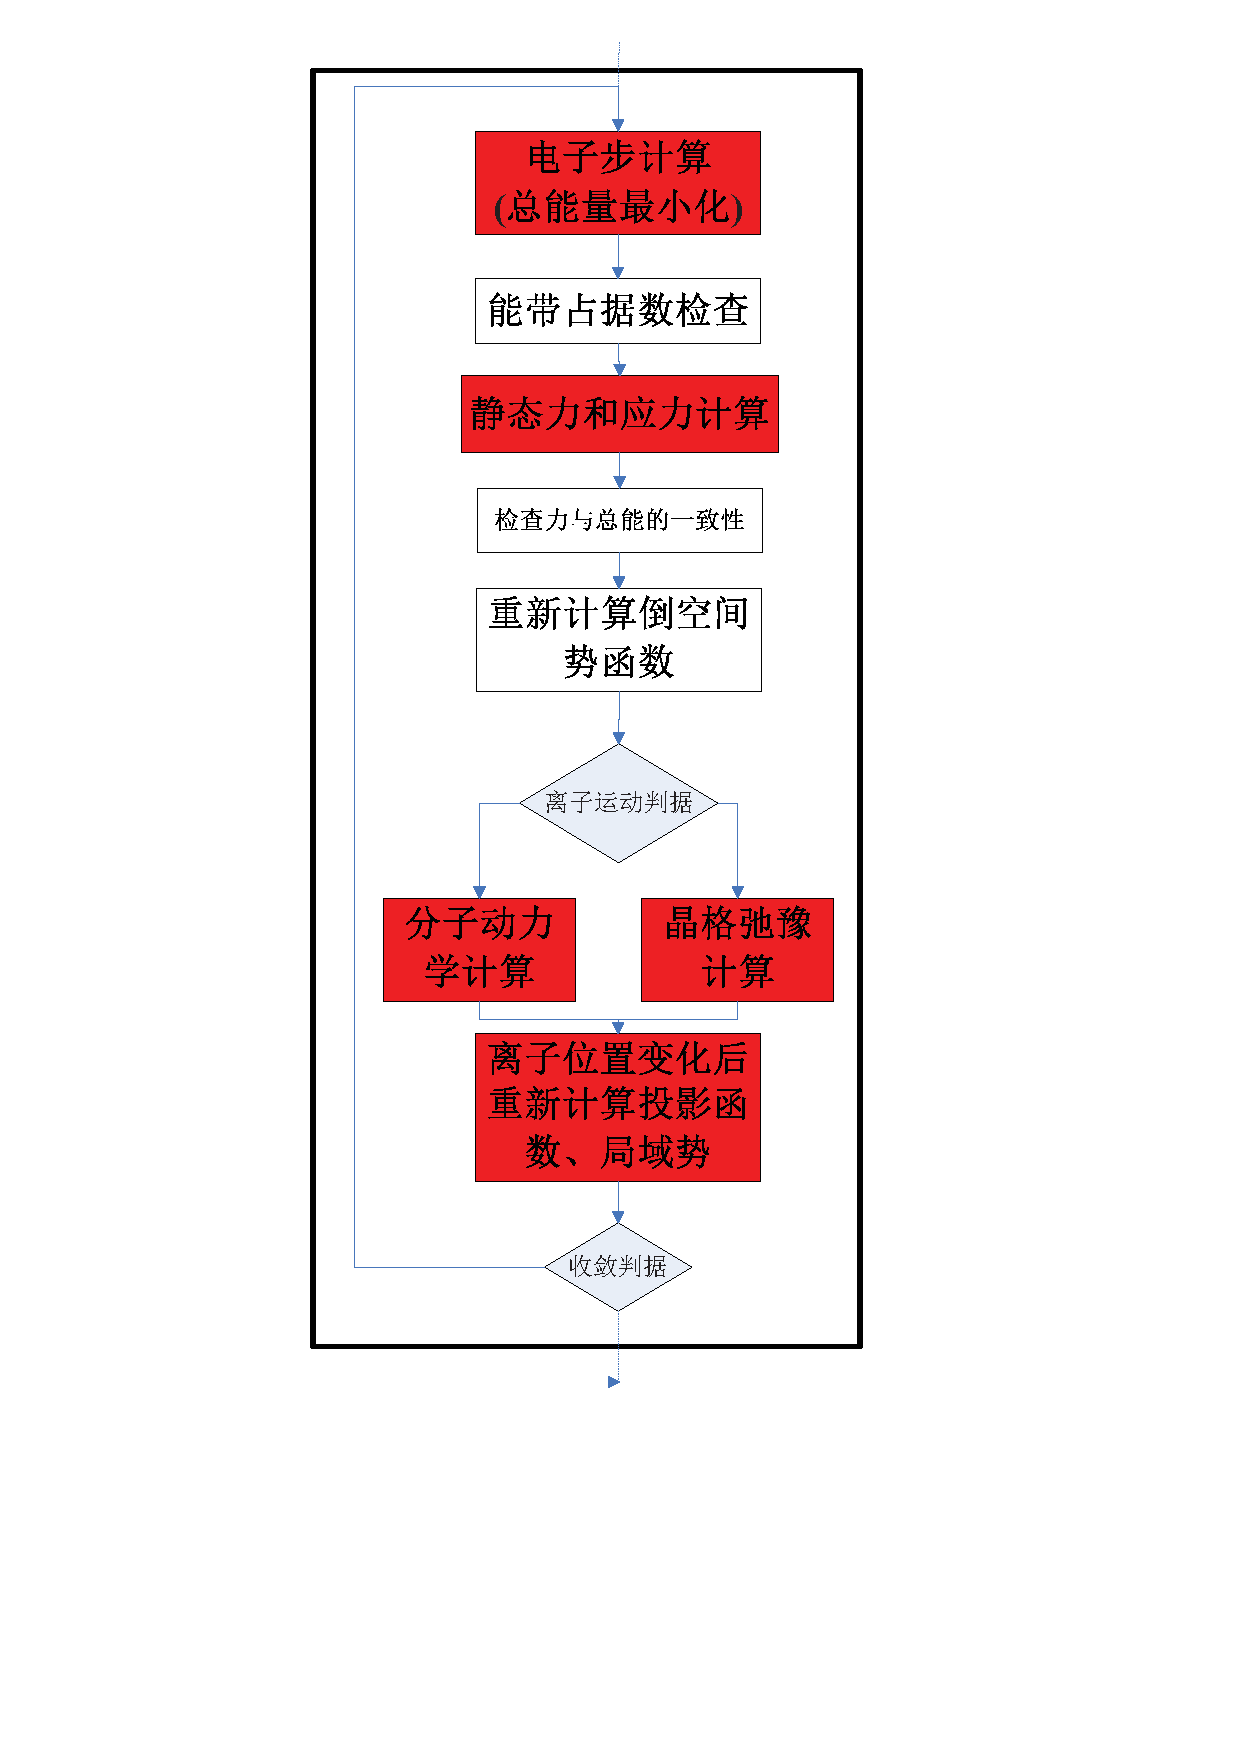
\includegraphics[height=2.30in,width=4.0in,viewport=0 0 562 350,clip]{Figures/VASP_main_Flow-3.png}
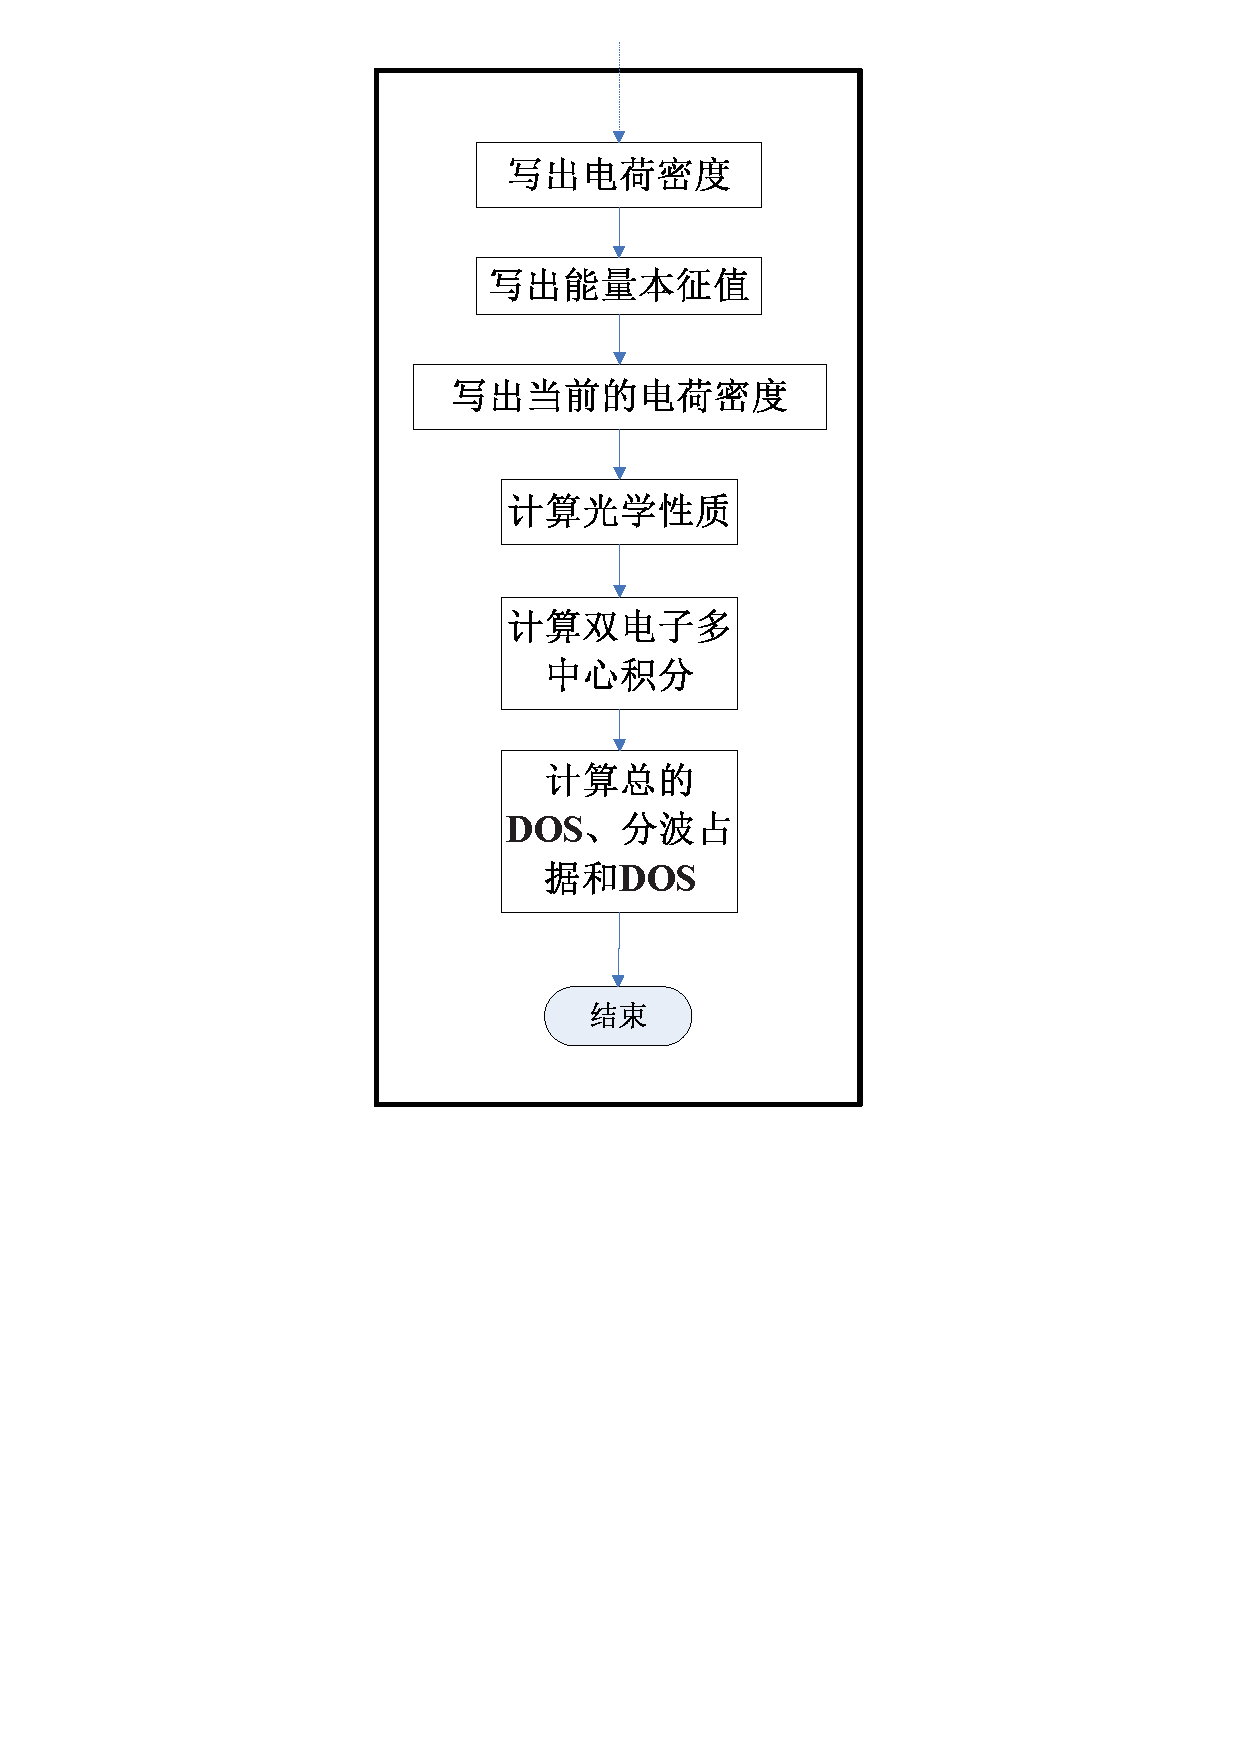
\includegraphics[height=2.10in,width=4.0in,viewport=0 215 562 530,clip]{Figures/VASP_main_Flow-4.png}
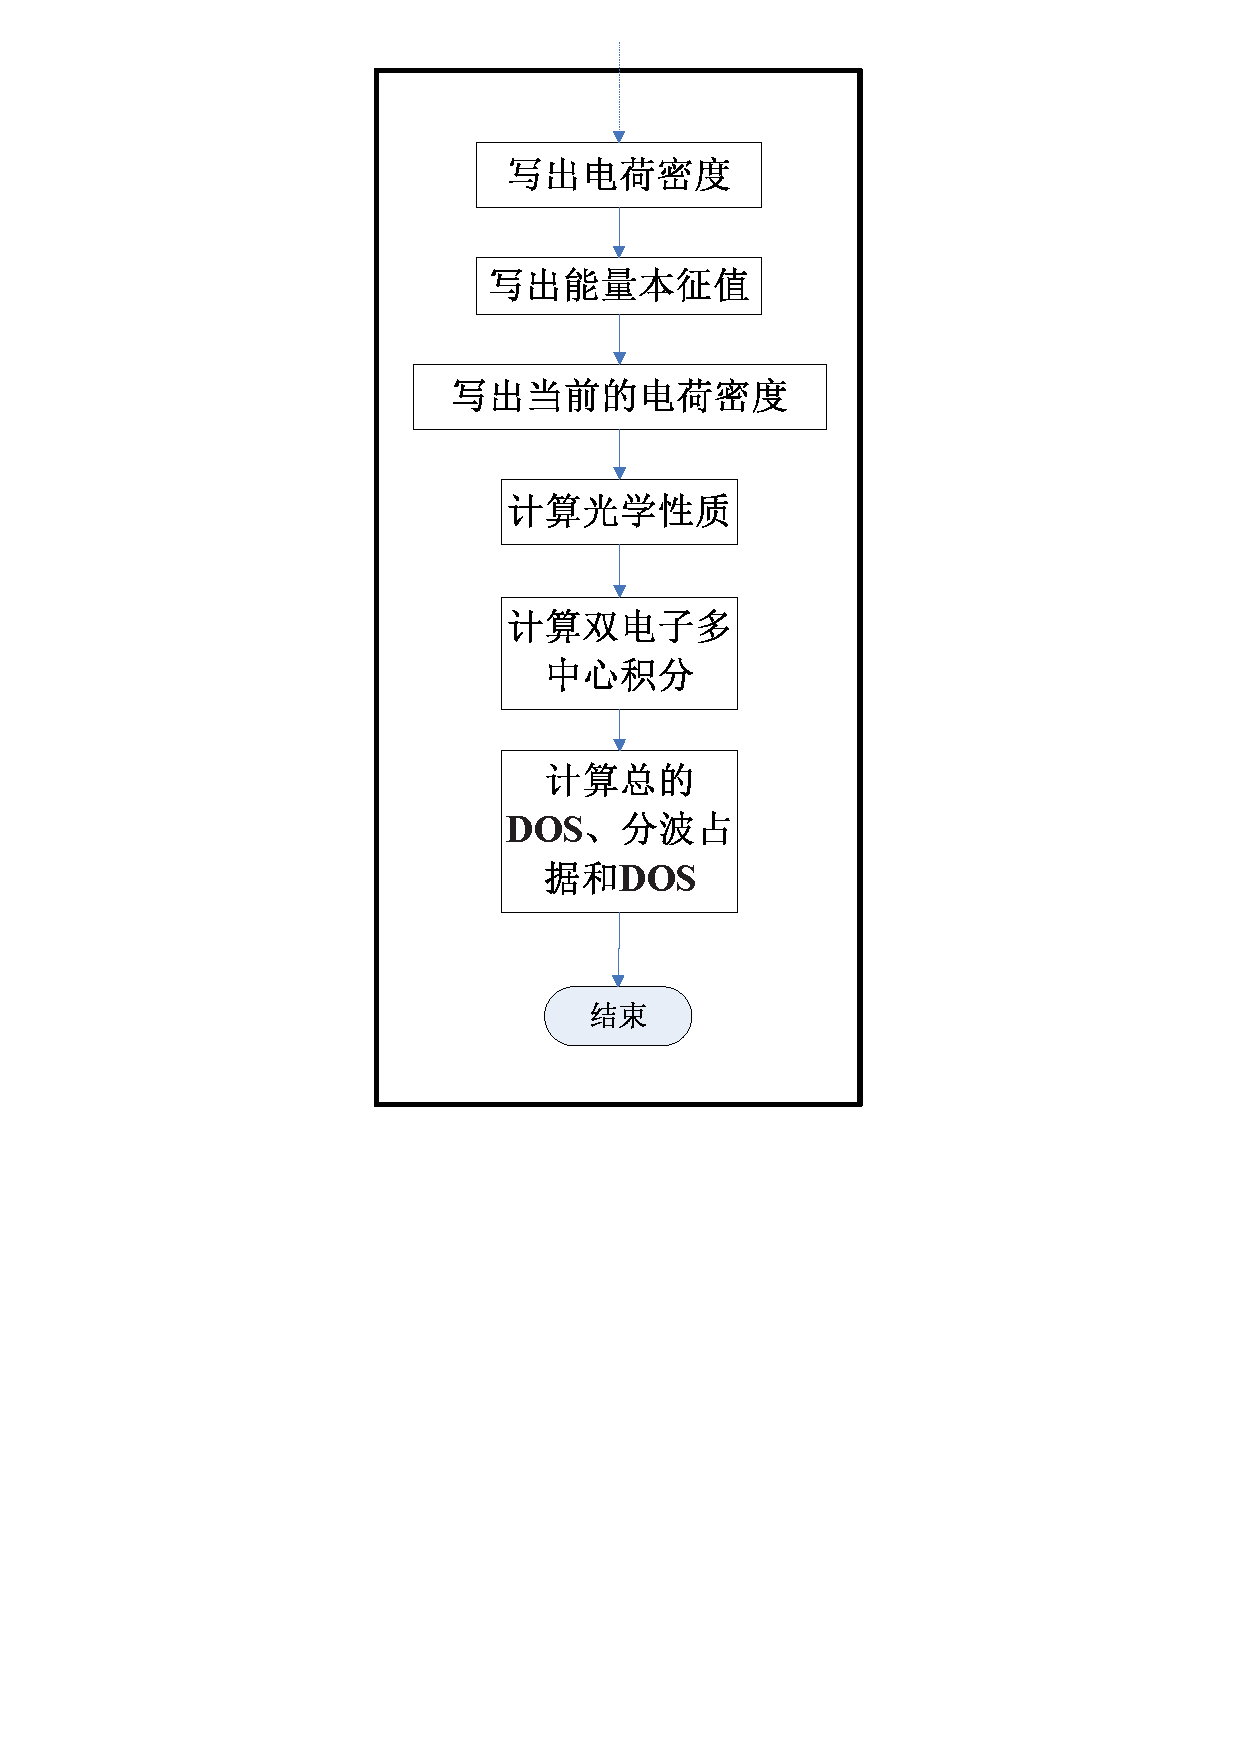
\includegraphics[height=1.30in,width=4.0in,viewport=0 0 562 215,clip]{Figures/VASP_main_Flow-4.png}
\caption{\tiny \textrm{Creators of DFT. Walter Kohn(left, in 1962) and his two postdoctoral fellows, Pierre Hohenberg (middle, in 1965) and Lujeu Sham (right).}}%(与文献\cite{EPJB33-47_2003}图1对比)
\label{FLOW_of_VASP}
\end{figure}
\end{frame}
